%!TEX root = project.tex

\chapter*{About this project}
\paragraph{Analysis of this project: }
%ADD references TO MERN STACK AND PYTHON HERE
This project was designed by me for the module Applied Project \& Dissertation with the purpose being
to complete an online banking system using a MERN(Mongo, Express, React \& Node) stack.
The project should allow user to login, view statements, takeout loans, perform transactions and
will show the user there monthly and yearly expenditures using graphs. The project will also be
secure and utilize user accounts using a mongo Database to ensure that the users account is secure.
\\*
\\*
The main purpose of this project is to utilize the MERN stack to provide a full and rich user
experience and to provide a secure, intuitive and polished online banking system.  The project
will also utilize Python scripts to perform statistical analysis on user expenditure and income
and will provide an estimate of how much money the user should have for the month based upon previous
monthly expenditure.
\\*
\\*
This project was designed to be a stand alone application where a user can perform all their
banking needs without any other software.  The user should be find the UI intuitive and the
features helpful.
\\*
\\*
This project will link many disparate technologies together for the purpose of providing the user
with the features they need.  I plan to use this project to show the skills I have attained during
my course and to learn a new framework(React). I also plan to improve and cultivate my skills
using new technologies such as various Python libraries and React. This project is stored on a GitHub
repository the link to which is found in the \nameref{gitLink}
\paragraph{Authors: }
My name is \textbf{Ultan Kearns}, I am a fourth year student at GMIT. I have never used
React or \LaTeX\  before but I plan to learn a lot about these technologies during the course of this project.


\chapter{Introduction}
%Make sure you use references
\section {Why A MERN stack?}
\begin{center}

\includegraphics[width=\textwidth]{img/mern.jpeg}
\end{center}
There are many reasons why I have chosen to use a MERN stack for this
application the main one is because it provides a framework for a full stack
application.
MERN stands for \textbf{Mongo - For the database backend(Hosted on Mlab, all user info is stored here),
Express - A web application framework
host a server in a relatively short time compared to other methods
, ReactJS for asynchronous JS \& Node - for package management.}
\cite{https://www.mongodb.com/blog/post/the-modern-application-stack-part-1-introducing-the-mean-stack}
\\
\subsection{Mongo}
As you have read above the MERN stack is very powerful in creating a full-stack
application when used correctly.  The reason I chose the database Mongo is because
it offers an open source alternative to MySQL and other proprietary databases
\cite{https://www.educba.com/mongodb-open-source/}
and many companies seem to be migrating to it because it is open source and in
some cases may offer better performance than other databases.
\begin{center}
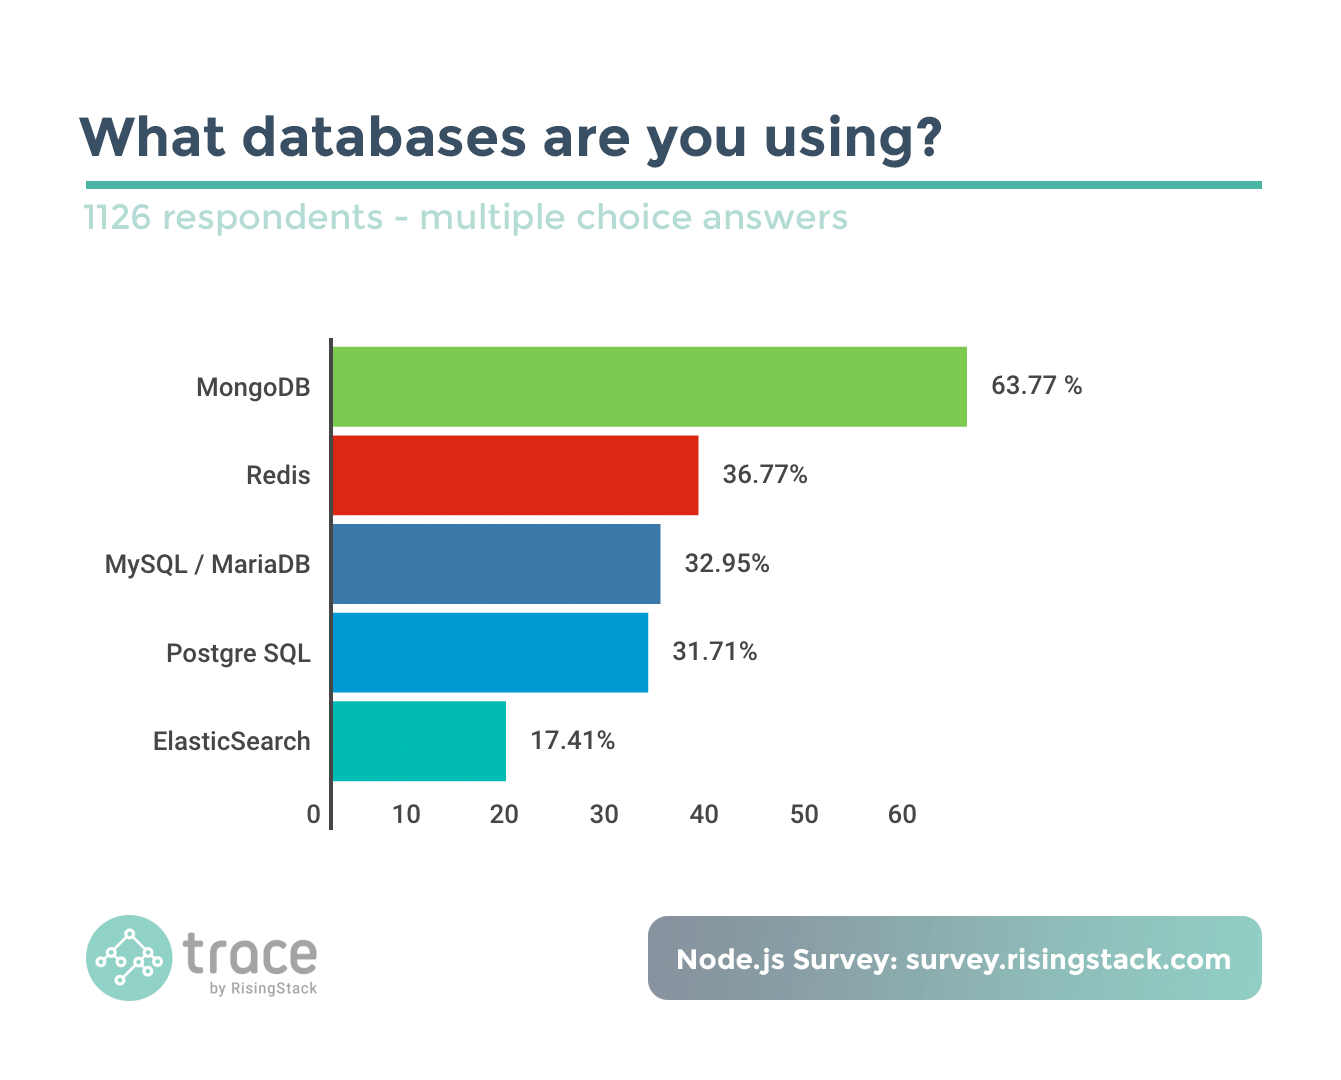
\includegraphics[width=\textwidth]{img/mongostat.png}
\end{center}
\cite{https://blog.risingstack.com/node-js-developer-survey-results-2016/}
Mongo is easy to learn as it stores it's data in JSON format and is schemaless, that is the user
defines their own schemas. I have also used it for 2 other projects in Angular and find it an
easy database to use in relation to projects.
\\
\subsection{Express}
I chose to use Express because it is a very useful API when creating a server.
It is very helpful when pulling data from the server and displaying it to the client
it is also very scalable and offers good security when used properly.  It is also very
easy to setup and can be connected to the MLab database in minutes upon starting the
project.  I have also used this server before and have a bit of experience with it and
found it very helpful in the projects I used it for which were a messaging forum and an
E-commerce application both using MEAN(Mongo,Express,Angular \& Node) stacks.
\\
\subsection{React}
I also chose this project because I have zero experience in ReactJS and since
it's such an up and coming framework I decided on it for this project. It also
offers many features and libraries which are desirable when programming a user
interface to ensure the user finds the application intuitive and easy to use.
ReactJS also utilizes modular programming for components which makes designing
web applications far easier than just using HTML, CSS \& Javascript. React is
also very fast at rendering pages so that the user will not experience a major
delay in accessing information.
\\
\subsection{Node}
The reason I chose Node Package Manager was because it offers many great packages which can be
used to improve productivity on my part and also the applications security, UI,
UX and various other aspects of the application.  I debated using Yarn for this
project but settled on Node because it was already installed on my laptop.  Node
is a very useful tool when developing full-stack applications and was very helpful
in installing tools and libraries for react.
\section{Why a banking application?}
\subsection{Explanation of why I chose this project}
A banking application is broad in scope and offers many questions to the developer
such as how can I optimize load times and how can I ensure user data is secure.
I think questions such as these offer the potential for growth in the areas of
design and problem solving - which are two of the most major skills a software
developer can possess. I feel that an application such as a multi-user banking
system can be beneficial to my career and help to improve my skills as a developer.
Banking applications also have the potential to offer a wide array of features and
are ubiquitous in the real world, think major banks such as AIB \& Bank of Ireland.
Banking systems also offer a broad range of problems such as security, design
and usability.
\\
\subsection{My Contention with existing online banking systems \& how I plan to improve upon them}
The current generation of online banking systems or at least the ones I have used
tend to have a variety of problems.  These problems are glaringly obvious to most
people and the main problems include but are not limited to: usability, appearance, lack of
personalization \& lack of information given to user.  I will how I plan to solve each of
these problems below:
\begin{itemize}
\item \textbf{Usability:} I aim to provide an intuitive and cutting-edge user
interface using the latest react libraries to provide the user with an easy to
understand banking application.  All features will be easily navigated to using
a navigation bar and I will aim to make features as obvious as possible to the user.
\item \textbf{Appearance:} The UI of the modern day online banking system tends
to be absolutely depressing.  I aim to reduce this by adding in a responsive UI
and to offer the user a vibrant online banking experience.
\item \textbf{Lack of personalization:} I aim to make this application very personal
to the user by adding in personalized expenditure charts and giving the user a
unique and inimitable banking experience.
\item \textbf{Lack of information:} Modern banking applications sometimes display
a lack of information given to the user.  I plan to solve this by offering the user
expenditure charts, reports and also by sending automated emails to them when
their account balance falls below a user specified number.
\end{itemize}
\section{Requirements}
Below I will include the requirements for this application and expand upon them.
\begin{itemize}
\item \textbf{Multiple Users:} This application must allow multiple users to
execute simultaneous banking and user sessions must be independent of each
other.
\item \textbf{Secure:} Database information must be encrypted
\item \textbf{Accurate:} All statments and user information must be accurate.
\item \textbf{Login/Logout} The user must be able to login and logout
\item \textbf{information}: The user must be able to view all information related
to them (eg: statments, withdrawl dates etc.)
\item \textbf{Graphs/Charts}: The banking app must display expenditures and
credit in graphs and charts generated from python scriptss
\item \textbf{Emails} The application must be able to email the user a forgot
password if they forgot their password and alos be able to email the user if
budget controls are turned on.
\item \textbf{Register} The user must be able to register new accounts using
an email and password also ensure that it cannot be an email that already exists.
\item \textbf{Delete account} The user must be able to terminate their account
and all information that exists about the user must be purged from the server.
\item \textbf{Change information} The user must be able to update all their personal
information in relation to their account except obviously banking statments and
balances.
\item \textbf{User sessions} The application must use cookies to maintain a
user session and ensure that the cookies do not last more than a specified timeframe
max of a day.
\end{itemize}

\chapter{Context}
\begin{itemize}
\item Provide a context for your project.
\section{Project Objectives}
\begin{itemize}
  \item To provide safe \& secure online banking
  \item To provide an intuitive UI that can be easily navigated by the user
  \item To provide user generated statistical analysis of expenditure
  \item To provide a multi-user server and banking service
  \item To provide a RESTful API to the banking service(client/server totally independent
  ,stateless environment, caching)
  \item To provide a scalable application
  \item To provide user with security using encryption for the mongo database
  \item To limit loadtimes of traditional online banking eg. 365 Online Banking and others
\end{itemize}
\item Briefly list each chapter / section and provide a 1-2 line description of what each section contains.
\item List the resource URL (GitHub address) for the project and provide a brief list of the main elements at the URL.
\end{itemize}

\section{Filler}
Lorem ipsum dolor sit amet, consectetur adipiscing elit. Etiam mi enim, interdum ut elit lobortis, bibendum tempus diam. Etiam turpis ex, viverra tristique finibus nec, feugiat at metus. Curabitur tempus gravida interdum. Donec ac felis a lorem scelerisque elementum. Vestibulum sit amet gravida tortor, a iaculis orci. Nam a molestie augue. Curabitur malesuada odio at mattis molestie. In hac habitasse platea dictumst. Donec eu lectus eget risus hendrerit euismod nec at orci. Praesent porttitor aliquam diam, eu vestibulum nisl sollicitudin vel. Nullam sed egestas mi.

Quisque vel erat a justo volutpat auctor a nec odio. Sed rhoncus augue sit amet nisl tincidunt, vitae cursus tellus efficitur. Class aptent taciti sociosqu ad litora torquent per conubia nostra, per inceptos himenaeos. Pellentesque et auctor dui. Fusce ornare odio ipsum, et laoreet mi molestie sed. Cras at massa sit amet ipsum gravida aliquam. Nulla suscipit porta imperdiet. Fusce eros neque, bibendum sit amet consequat non, pulvinar quis ipsum.

\subsection{More filler}
Donec fermentum sapien ac rhoncus egestas. Nullam condimentum condimentum eros sit amet semper. Nam maximus condimentum ligula. Praesent faucibus in nisi vitae tempus. Sed pellentesque eleifend ante, ac malesuada nibh dapibus nec. Phasellus nisi erat, pulvinar vel sagittis sed, auctor et magna. Quisque finibus augue elit, consequat dignissim purus mollis nec. Duis ultricies euismod tortor, nec sodales libero pellentesque et. Interdum et malesuada fames ac ante ipsum primis in faucibus.

Donec id interdum felis, in semper lacus. Mauris volutpat justo at ex dignissim, sit amet viverra massa pellentesque. Suspendisse potenti. Praesent sit amet ipsum non nibh eleifend pretium. In pretium sapien quam, nec pretium leo consequat nec. Pellentesque non dui lacus. Aenean sed massa lacinia, vehicula ante et, sagittis leo. Sed nec nisl ac tellus scelerisque consequat. Ut arcu metus, eleifend rhoncus sapien sed, consequat tincidunt erat. Cras ut vulputate ipsum.

Curabitur et efficitur augue. Proin condimentum ultrices facilisis. Mauris nisi ante, ultrices sed libero eget, ultrices malesuada augue. Morbi libero magna, faucibus in nunc vitae, ultricies efficitur nisl. Donec eleifend elementum massa, sed eleifend velit aliquet gravida. In ac mattis est, quis sodales neque. Etiam finibus quis tortor eu consequat. Nullam condimentum est eget pulvinar ultricies. Suspendisse ut maximus quam, sed rhoncus urna.

\section{Filler}
Phasellus eu tellus tristique nulla porttitor convallis. Vestibulum ac est eget diam mollis consectetur. Donec egestas facilisis consectetur. Donec magna orci, dignissim vel sem quis, efficitur condimentum felis. Donec mollis leo a nulla imperdiet, in bibendum augue varius. Quisque molestie massa enim, vitae ornare lacus imperdiet non. Donec et ipsum id ante imperdiet mollis. Nullam est est, euismod sit amet cursus a, feugiat a lectus. Integer sed mauris dolor.

Mauris blandit neque tortor, consequat aliquam nisi aliquam vitae. Integer urna dolor, fermentum ut iaculis ut, semper eu lacus. Curabitur mollis at lectus at venenatis. Donec fringilla diam ac risus imperdiet suscipit. Aliquam convallis quam vitae turpis interdum, quis pharetra lacus tincidunt. Nam dictum maximus lectus, vitae faucibus ante. Morbi accumsan velit nec massa tincidunt porttitor. Nullam gravida at justo id viverra. Mauris ante nulla, eleifend vitae sem vitae, porttitor lobortis eros.

Cras tincidunt elit id nisi aliquam, id convallis ex bibendum. Sed vel odio fringilla, congue leo quis, aliquam metus. Nunc tempor vehicula lorem eu ultrices. Curabitur at libero luctus, gravida lectus sed, viverra mi. Cras ultrices aliquet elementum. Pellentesque habitant morbi tristique senectus et netus et malesuada fames ac turpis egestas. Sed metus ante, suscipit sit amet finibus ut, gravida et orci. Nunc est odio, luctus quis diam in, porta molestie magna. Interdum et malesuada fames ac ante ipsum primis in faucibus. Mauris pulvinar lacus odio, luctus tincidunt magna auctor ut. Ut fermentum nisl rhoncus, tempus nulla eget, faucibus tortor. Suspendisse eu ex nec nunc mollis pulvinar. Nunc luctus tempus tellus eleifend porta. Nulla scelerisque porttitor turpis porttitor mollis.

Duis elementum efficitur auctor. Nam nisi nulla, fermentum sed arcu vel, posuere semper dui. Fusce ac imperdiet felis. Aenean quis vestibulum nisl. Integer sit amet tristique neque, at suscipit tortor. Morbi et placerat ante, vel molestie dui. Vivamus in nibh eget massa facilisis accumsan. Nunc et purus ac urna fermentum ultrices eget sit amet justo. Class aptent taciti sociosqu ad litora torquent per conubia nostra, per inceptos himenaeos. Cras elementum dui nunc, ac tempor odio semper et. Ut est ipsum, sollicitudin eleifend nisl eu, scelerisque cursus nunc. Nam at lectus vulputate, volutpat tellus vel, pharetra mauris. Integer at aliquam massa, at iaculis sem. Morbi nec imperdiet odio. In hac habitasse platea dictumst.

Mauris a neque lobortis, venenatis erat ut, eleifend quam. Nullam tincidunt tellus quis ligula bibendum, a malesuada erat gravida. Phasellus eget tellus non risus tincidunt sagittis condimentum quis enim. Donec feugiat sapien sit amet tincidunt fringilla. Vivamus in urna accumsan, vehicula sem in, sodales mauris. Aenean odio eros, tristique non varius id, tincidunt et neque. Maecenas tempor, ipsum et sollicitudin rhoncus, nibh eros tempus dolor, vitae dictum justo massa in eros. Proin nec lorem urna. In ullamcorper vitae felis sit amet tincidunt. Maecenas consectetur iaculis est, eu finibus mi scelerisque et. Nulla id ex varius, ultrices eros nec, luctus est. Aenean ac ex eget dui pretium mattis. Ut vitae nunc lectus. Proin suscipit risus eget ligula sollicitudin vulputate et id lectus.


\chapter{Methodology}
About one to two pages.
Describe the way you went about your project:
\begin{itemize}
\item Agile / incremental and iterative approach to development. Planning, meetings.
\item What about validation and testing? Junit or some other framework.
\item If team based, did you use GitHub during the development process.
\item Selection criteria for algorithms, languages, platforms and technolo-gies.
\end{itemize}
Check out the nice graphs in Figure %\ref{tikz:graphs}, and the nice diagram in Figure %\ref{tikz:mydiagram}.

\begin{figure}
  \centering
  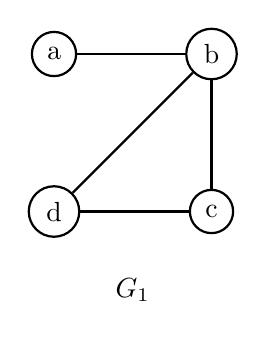
\begin{tikzpicture}
  \begin{scope}[every node/.style={circle,thick,draw}]
  \node (a) at (0,2) {a};
  \node (b) at (2,2) {b};
  \node (c) at (2,0) {c};
  \node (d) at (0,0) {d};
  \end{scope}
  \begin{scope}[every edge/.style={draw=black,thick}]
  \path (a) edge (b);
  \path (b) edge (c);
  \path (b) edge (d);
  \path (c) edge (d);
  \end{scope}
  \node () at (1,-1) {$G_1$};
  \end{tikzpicture}
  \hspace{1.5cm}
  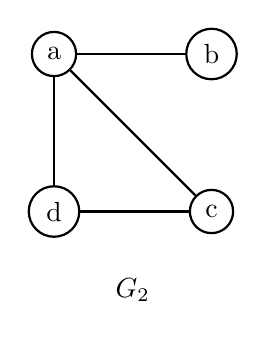
\begin{tikzpicture}
  \begin{scope}[every node/.style={circle,thick,draw}]
  \node (1) at (0,2) {a};
  \node (2) at (2,2) {b};
  \node (3) at (2,0) {c};
  \node (4) at (0,0) {d};
  \end{scope}
  \begin{scope}[every edge/.style={draw=black,thick}]
  \path (1) edge (2);
  \path (1) edge (3);
  \path (1) edge (4);
  \path (3) edge (4);
  \end{scope}
  \node () at (1,-1) {$G_2$};
  \end{tikzpicture}
  \caption{Nice pictures}
  \label{tikz:graphs}
\end{figure}


\begin{figure}
  \centering
  \begin{tikzpicture}[node distance=6cm]
  \node (a) [rect] {A Big Blue Block};
  \node (b) [oval, right of=a] {And His Oval Friend};
  \draw [line] (a) -- (b);
  \end{tikzpicture}
  \caption{Nice pictures}

\end{figure}


\chapter{Technology Review}
About seven to ten pages.
\begin{itemize}
\item Describe each of the technologies you used at a conceptual level. Standards, Database Model (e.g. MongoDB, CouchDB), XMl, WSDL, JSON, JAXP.
\item Use references (IEEE format, e.g. [1]), Books, Papers, URLs (timestamp) – sources should be authoritative.
\end{itemize}

\section{XML}
Here's some nicely formatted XML:
\begin{minted}{xml}
<this>
  <looks lookswhat="good">
    Good
  </looks>
</this>
\end{minted}

\chapter{System Design}
As many pages as needed.
\begin{itemize}
\item Architecture, UML etc. An overview of the different components of the system. Diagrams etc… Screen shots etc.
\end{itemize}

\begin{table}[h]
  \centering
  \begin{tabular}{x{2cm}p{3cm}}
    \toprule \\
    Column 1 & Column 2 \\
    \midrule \\
    Rows 2.1 & Row 2.2 \\
    \bottomrule
  \end{tabular}
  \caption{A table.}
  \label{table:mytable}
\end{table}

\chapter{System Evaluation}
As many pages as needed.
\begin{itemize}
\item Prove that your software is robust. How? Testing etc.
\item Use performance benchmarks (space and time) if algorithmic.
\item Measure the outcomes / outputs of your system / software against the objectives from the Introduction.
\item Highlight any limitations or opportuni-ties in your approach or technologies used.
\end{itemize}

\chapter{Conclusion}
About three pages.
\begin{appendices}
\chapter{Preamble \& Intro}
\begin{itemize}
  \label{gitLink}
\item \href{https://github.com/Ultan-Kearns/AppliedProject}{Link to my github}
\hfill
\hyperlink{page.3}{Go to page 3}
\end{itemize}
\end{appendices}
\end{document}
